%AXIOMATIC MODEL DEMYSTIFIED----------------------------------------------

\documentclass[10pt]{article}
\usepackage[utf8]{inputenc}
\usepackage{amsmath}
\usepackage{amssymb}
\usepackage[a4paper,margin=1in,footskip=0.25in]{geometry}
\usepackage[dvipsnames]{xcolor}
\usepackage{graphicx}
\usepackage{tikz}
\usepackage{amsthm}
\usepackage{float}
\usepackage{centernot}

%Using tikz library for flowcharts and arrows
\usetikzlibrary{shapes.geometric, arrows}

%For proper positioning of flowchart nodes
\usetikzlibrary{positioning}

%Setting some preliminary shapes for flowchart and arrows
\tikzstyle{inst} = [draw = none, fill = none]
\tikzstyle{arrow} = [->, >=stealth, thin]

\tikzstyle{imply} = [->, thick, >=stealth]

\title{ECMAScript Axiomatic Memory Consistency Model}
\author{Akshay Gopalakrishnan}
\date{November 2019}

\begin{document}

\maketitle


%Short form to use stack_relative
\newcommand{\stck}{\stackrel{\longrightarrow}}

%A different version of the above 
\newcommand{\stckdet}[1]{\stackrel{{#1}}}

%We write a lot of relations between two events using the orderings, so a short form to use that
\newcommand{\reln}[3]{#1\stck{_{#2}}#3}

%We use a more detailed version of the above relation to indicate direct / indirect relations 

\newcommand{\reldet}[4]{#1\stckdet{_{#2}}{{\stck{_{#3}}}}#4}

%We also will introduce a short form to write an event belongs to some set
\newcommand{\event}[2]{#1\!\in\!#2}

%To make events and their type more close to each other
\newcommand{\typ}[1]{\textit{#1}}
\newcommand{\et}[2]{#1\!:\!\typ{#2}}

%Short form to write color text
\newcommand{\critic}[2]{\textcolor{#1}{\footnotesize #2}}

%COMMENT FOR NOW AS IT IS NOT OUR PRIORITY 
%
\section{Introduction}
    Instruction reordering is a common transformation done by the compiler/hardware, which is essential to optimizations such as instruction scheduling, loop invariant removal, partial redundancy elimination, etc. 
    However, whether we can do such reordering freely given a concurrent program using relaxed memory accesses is a bit unclear. 
     
    \paragraph{Simple reordering is not straightforward under shared memory semantics}
    The main reason is that memory accesses here, do not just perform the desired operation (i.e Read / Write) but also imply certain visibility guarantees across all the other threads.  
    In our observation, we find that, the relaxed memory model of ECMAScript prescribe semantics for visibility using the $\stck{_{hb}}$ relations. 
    
    \paragraph{Some Examples}
        We show a couple of examples to showcase why reordering may not be that straightforward. 
        Consider the first example in Figure~\ref{reord:example1(a)} below of a Candidate before and after reordering two events.
        The original candidate is to the left and that on the right is after reordering the two reads of $T2$.
        The observable behavior in question is written in the middle(orange box). 
        \begin{figure}[H]
            \centering
            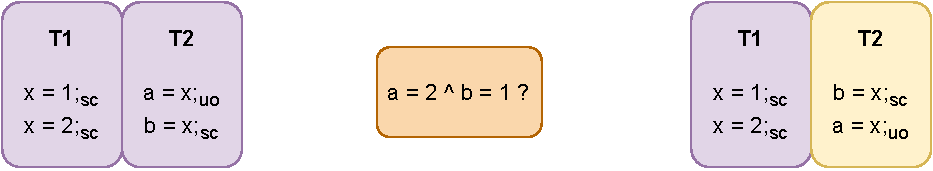
\includegraphics[scale=0.7]{5.InstructionReordering/0.Intro/ReorderingExample1(a).pdf}
            \caption{First example for reordering in candidates of the original program and its reordered counterpart.}
            \label{reord:example1(a)} 
        \end{figure}
        
        Figure~\ref{reord:example1(b)} has two sets of relations. 
        The first justifies the outcome for the reordered Candidate. 
        While the second justifies for the original Candidate. 
        Notice that in the first set of relations, we can infer that one may have a read memory ordered before a write that it reads from. 
        This is quite counter intuitive to understand at first. 
        But strictly from the semantics of the model, this justification to the observable behavior is completely valid\footnotemark. 
        \begin{figure}[H]
            \centering
            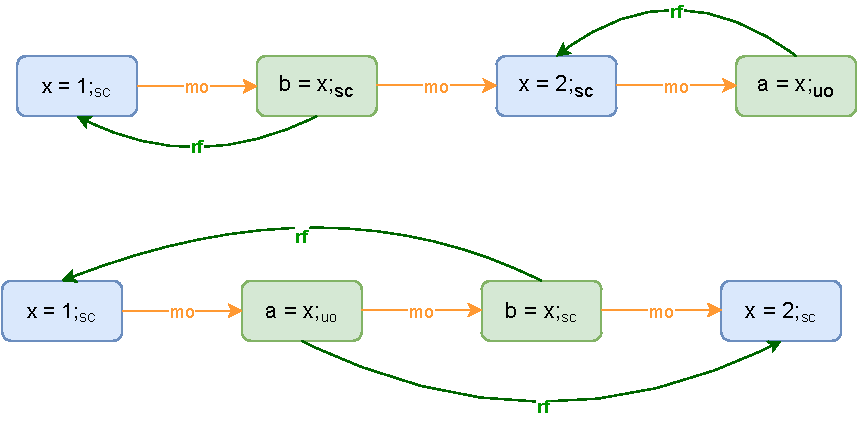
\includegraphics[scale=0.7]{5.InstructionReordering/0.Intro/ReorderingExample1(b).pdf}
            \caption{The set of partial order relations justifying the observable behavior in question for both the candidates in Figure~\ref{reord:example1(a)}.} 
            \label{reord:example1(b)}
        \end{figure}

        \footnotetext{In practice, this can be due to read speculation at the hardware level.}
        
        Consider another example in Figure~\ref{reord:example2(a)}.
        The figure on the left is the original candidate and that on the right is after reordering the two events of $T1$.
        The observable behavior in question is written in the middle(orange box). 
        \begin{figure}[H]
            \centering
            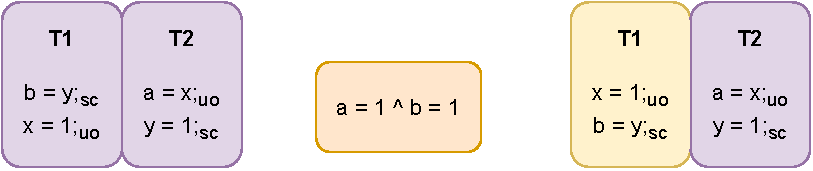
\includegraphics[scale=0.7]{5.InstructionReordering/0.Intro/ReorderingExample2(a).pdf}
            \caption{Second example for reordering with candidates of the original program and its reordered counterpart.} 
            \label{reord:example2(a)}
        \end{figure}
   
        Figure~\ref{reord:example2(b)} has two sets of relations. 
        The first justifies that such an outcome is not possible for the original program candidate due to Axiom \ref{CoRe}. 
        While the second justifies that this outcome is possible for the reordered program.
        Note that we cannot infer in the reordered candidate the set of relations for any candidate execution to have $\reln{a=x;_{uo}}{hb}{x=1;_{uo}}$. 
        \begin{figure}[H]
            \centering
            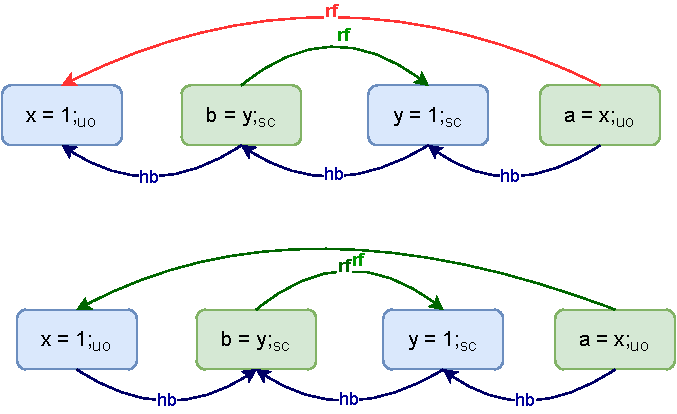
\includegraphics[scale=0.7]{5.InstructionReordering/0.Intro/ReorderingExample2(b).pdf}
            \caption{The set of partial order relations justifying the observable behavior in question for both the candidates in Figure~\ref{reord:example2(a)}.} 
            \label{reord:example2(b)}
        \end{figure}

        The above two examples show that we have to be careful while reordering two events in the same thread. 
        By example analysis, for each observable behavior, one must check all possible candidate executions and assert whether such an observable is possible or not. 
        This method of checking validity of reordering will scale exponentially as the program size increases. 
        It may also be the case that the compiler may not have information on which exact events would be executed in other threads to assert such reordering is valid. 

    
    
    
    
    


%The ECMAScript Memory Model

%AGENTS----------------------------------------------------------------------------------------------------------------------------------------  
\section{Agents, Events and their Types}

    \subsection{Agents}
        A concurrent program involves different threads/processes running concurrently. Agents are analogous to different threads/processes. 
        
        \critic{red}{Agents actually have more meaning than what we refer to here. However, in terms of reasoning just with memory consistency rules, we are safely abstracting them to just mean threads/processes.}

        %Agent Clusters
        \paragraph{Agent Cluster}
        Collection of agents concurrently communicating with each other (directly/ indirectly) form an agent cluster.  There can be multiple agent clusters. However, an agent can only belong to one agent cluster.

        \critic{red}{Please look back at what Conrad had said to about agent clusters.}
        
        %Perhaps give an example here later

        \critic{blue}{Note that for the purpose of reasoning with optimizations given the memory model, we stick to assuming that just one agent cluster exists. We also assume that agents in the cluster communicate only through one common shared memory segment.}

        \critic{purple}{Could elaborate the role when different shared array buffers are used to communicate accross agents belonging to different clusters. However, this is something that is not primary to our purpose of investigation, but would be essential as a whole from a practical standpoint to enforce correct concurrent programming.}
        
        %Agent Event Set
        \paragraph{Agent Event List $(ael)$}
        Every agent is mapped to a list of events. Operationally (when a program actually runs),  these events are appended to the list during evaluation. We define $ael$ is a mapping of each agent to a list of events.
        
            \[ael(a) = [e_1, e_2, ... e_k ] \]
        
        \critic{blue}{The standard refers this to be an Event List, but we find it a bit misleading as it does not signify a list for each agent. Hence we name it as Agent Event List}

        

            



%Events------------------------------------------------------------------
    \subsection{Events}
        
        An evaluation of an operation results in a set of events that are evaluated. An event is either an operation that involves (shared) memory access or that constrains the order of execution of multiple events. The latter are called \textit{Synchronize Events}

        \critic{blue}{Synchronizing events are analogous to $lock$ and $unlock$ events that allow exclusive access to critical sections of memory.}  

%Events----------------------------------------------------------------------------------------------------------------------------------
    
    %Useful command syntax
    \newcommand{\rmw}{\textit{rmw}\,}
    \newcommand{\set}[1]{\textbf{\textit{#1}}}

%Events------------------------------------------------------------------
    \subsection{Events}
    Agent execution is modelled in terms of events. 
    An event, in our context, is either an operation that involves (shared) Read/Write memory access or Synchronize events that constrains the order of execution of multiple events. 
    We define \set{E} as the set of events involved in an agent cluster. 
    We refer to \set{SM}, \set{R}, \set{W}, \set{S} as sets of Shared Memory, Read, Write and Synchronize events respectively. Read-Modify-Write events belong to both \set{R} and \set{W}. 
       
        \subsubsection{Range ($\Re$)}
            Each of the \textit{shared memory events} are associated with a contiguous range of memory on which it operates. $\Re$ is a function that maps a shared memory event to the range of memory indices it operates on which we represent as a starting index $i$ and a size $s$. As an example, the range of event $e$ would be like: 
                    
                    \[\Re(w) = (i, s) \]
           
            %\critic{red}{The range as per the ECMAScript standard denotes only the set of contiguous byte indices. The starting byte index is kept separate. We find this to be unnecessary. Hence we define range to have starting index and size.}
           
            We define two binary operators $\cap_\Re$ and $\cup_\Re$ to give the intersection and union respectively of the set of the byte indices, in order to describe disjoint, overlapping and equal ranges.  
            
%Types of Events Based on Order--------------------------------------------------------------------------------------------------------------------
    \subsubsection{Types of events based on Order} 
        There are 3 types (or access modes) which play a role in the sequence in which event actions are visible to different agents
        \begin{enumerate}
            \item \textbf{Sequentially Consistent ($sc$)} - Events of this type are $atomic$ in nature. There is a strict global total ordering of such events which is agreed upon by all agents in the agent cluster. 
            
            \item \textbf{Unordered ($uo$)} - Events of this type are considered non-atomic and can occur in different orders for each agent.
            
            \item \textbf{Initialize ($init$)} - Events of this type are used to initialize the values in memory ordered before events in an agent cluster.
        \end{enumerate}
        
        All events of type \textit{init} are writes and all read modify write events are of type \textit{sc}.
        We represent the type of events in the memory consistency rules in the format ``$\textit{event} : \textit{type}$''. 
        When representing events in a figure, the type would be represented as a subscript: $\textit{event}_\textit{type}$.
   
%Tearing factor of events
    \subsubsection{Tearing (or not)}
        Additionally, each shared-memory event is also associated with a tearing factor. 
        Events that tear are non-aligned accesses requiring more than one memory access. Events that are tear-free are aligned and should appear to be serviced in one memory access. The implication of tearing is better understood with the consistency rule that will later be shown.

%Relation among events----------------------------------------------------------------------------------------------------------------------------
    \subsection{Relation among events}
        We now describe a set of binary relations between events. These relations help us describe the consistency rules.
        
        \subsubsection{Read-Write event relations}
        There are two basic relations that assist us in reasoning about read and write events.
        
            %Read bytes from relation 
            \paragraph{Read-Bytes-From $(\stck{_{rbf}})$}
            
            This relation maps every read event to a list of tuples consisting of write event and their corresponding byte index that is read. For instance, consider a read event $r[i...(i+3)]$ and corresponding write events $w_1[i...(i+3)]$, $w_2[i...(i+4)]$. One possible $\stck{_\textit{rbf}}$ relation could be represented as  
                \begin{align*}
                    \reln{e}{\textit{rbf}}{\{(d1, i), (d2, i\!+\!1), (d2, i\!+\!2)\}}     
                \end{align*}   
            or having individual binary relation with each write-index pair as 
            \begin{align*}
                \reln{e}{rbf}{(d1, i)},\ \reln{e}{rbf}{(d2, i\!+\!1)}  \text{ and } \reln{e}{rbf}{(d2, i\!+\!2)}.
            \end{align*}
            
            %Reads from relation
            \paragraph{Reads-From $(\stck{_{rf}})$}
            
            This relation, is similar to the above relation, except that the byte index details are not involved in the composite list. So for the above example, the \textit{rf} relation would be represented either as   
                $\reln{e}{rf}{(d1, d2)}$
            or individual binary read-write relation as 
                $\reln{e}{rf}{d1}$ and $\reln{e}{rf}{d2}$.
            Figure below is an example of a program with its outcome (read values) shown in terms of reads-from relations. 
            \begin{figure}[H]
                \centering
                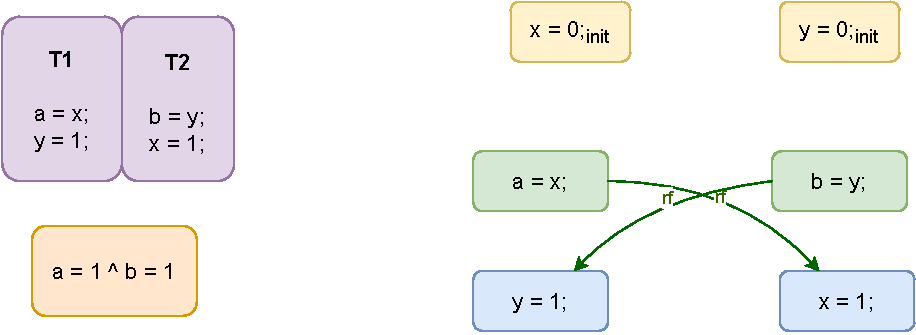
\includegraphics[scale=0.7]{ECMAScriptMemoryModel/ReadsFrom.pdf}
                \caption{An example to show the reads-from relations that are drawn for the example program between read and write events.}
                \label{read-from}
            \end{figure}
            
            %Agent sync with relation
        \subsubsection{Agent-Synchronizes With (\set{ASW})}
        
            It is a list for each agent that consist of ordered tuples of synchronize events. These tuples specify ordering constraints among agents at different points of execution. So such a list for an agent $k$ would be represented like:  
                \[ASW_k = \{ \langle s_1, s_2 \rangle, \langle s_3, s_4 \rangle ...\}\]
        
            For every pair in the list, the second event belongs to the parent agent and the first belongs to another agent it synchronized with\footnotemark.
                \[  
                    \forall{i,j>0},\ 
                    \langle s_1, s_2 \rangle \in ASW_j 
                    \Rightarrow{} 
                    s_2 \in ael(k)                        
                \]

            The figure below shows an example of this relation among two agents. 
            \begin{figure}[H]
                \centering
                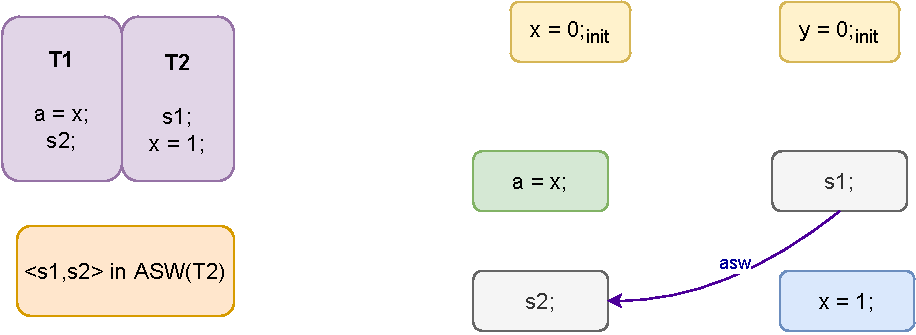
\includegraphics[scale=0.7]{ECMAScriptMemoryModel/AgentSyncWith.pdf}
                \caption{An example to show the reads-from relations that are drawn for the example program between read and write events.}
                \label{agent-sync-with}
            \end{figure}
        
        \footnotetext{This is analogous to the property that every unlock must be paired with a subsequent lock, which enforces the condition that a lock can be acquired only when it has been released.}

%Ordering Relation among Events----------------------------------------------------------------------------------------------------------------------       
        \section{Ordering Relations among Events}
        
        %Agent Order
        \paragraph{Agent Order ($\stck{_{ao}}$)}
            A total order among events belonging to the same agent event list. It is analogous to intra-thread ordering. For example, if two events $e$ and $d$ belong to the same agent event list , then either $\reln{e}{\textit{ao}}{d}$ or $\reln{d}{\textit{ao}}{e}$. 
            
            \critic{blue}{Note that the relations are only with respect to events belonging to the same agent. A collection of such relations together form the agent order. This is analogous to what we know as intra-thread sequential order. It is also the same as what \textbf{sequenced-before} is defined to be in C++.}

            \critic{purple}{Sequenced before maybe a bit weaker that agent order, as we saw in one of the papers. Basically, sequenced before precisely tells us which events can be reordered and which cannot, in contrast to agent order. I think it is similar to preserved program order in hardware, which is defined to capture dependancies resulting due to control flow in programs. Do check and see if these are the same. Discuss with Clark. }
        
        %Synchronize With Order
        \paragraph{Synchronize-With Order ($\stck{_{sw}} $)}
            Represents the synchronizations among different agents through relations between their events. It is a composition of two sets as below: 
            \begin{enumerate}
                \item All pairs belonging to $ASW$ of every agent belongs to this ordering relation. 
            
                        \[\forall{i, j > 0}, \ \langle e_i, e_j \rangle \in ASW \Rightarrow{} e_i \stck{_{sw}} e_j \]
            
                \item Specific reads-from pairs also belong to this ordering relation. 
            
                        \[(r \stck{_{rf}} w) \ \wedge \ \et{r}{sc} \ \wedge \ \et{w}{sc} \ \wedge \ (\Re(r)\!=\!\Re(w)) \ \Rightarrow{} \ (w \stck{_{sw}} r)\]
            
            \end{enumerate}
            
            \critic{blue} {Note that for the second condition, both ranges of events have to be equal. This however, does not mean that the read cannot read from multiple write events. (the read-from relation here is not functional.)}
            
        %Happens Before order 
        \paragraph{Happens Before Order ($\stck{_{hb}}$)}
            A transitive order on events, composed of the following:
            
            \begin{enumerate}
                \item Every agent-ordered relation is also a happens-before relation 
              
                    \[(e \stck{_{ao}} d) \ \Rightarrow{} \ (e \stck{_{hb}} d)\]
              
                \item Every synchronize-with relation is also a happens-before relation 
              
                    \[(e \stck{_{sw}} d) \ \Rightarrow{} \ (e \stck{_{hb}} d)\]
                     
                \item Initialize type of events happen before all shared memory events that have overlapping ranges with them. 
                
                    \[
                        \forall e,d \in SM \ \wedge \ 
                        \et{e}{init} \ \wedge \ 
                        (\Re(e) \cap \Re(d) \neq \phi)
                        \ \Rightarrow{} \ 
                        e \stck{_{hb}} d
                    \]
            \end{enumerate}
        
        \critic{red}{It is also important to note that those $\stck{_{hb}}$ relations that are formed due to Sequentially Consistent events (read-write), imply a more stronger visibility guarantee, in that all the threads observe the same global total order of such events. This however, is not expressed using this relation. Perhaps a better way to represent it may be required.}
        
        %Memory Order
        \paragraph{Memory Order ($\stck{_{mo}}$)}
            This order is a \textit{total order} on all events that respects happens-before order. 
                \[(e \stck{_{hb}} d) \Rightarrow{} (e \stck{_{mo}} d)\]
          

%Valid Execution Rules---------------------------------------------------------------------------------------------------------------------------------
    %MAKE SURE TO PLACE DEFINITONS ON PROGRAM, CANDIDATE, CANDIDATE EXECUTION and OBSERVABLE BEHAVIOURS        

    \subsection{Valid Execution Rules (the Axioms)}
        We now state the memory consistency rules. The rules are on \textit{Candidate Executions} which will place constraints on the possible \textit{Observable behaviors} that may result from it.
         
        %Coherent Reads   
        \subsubsection{Coherent Reads} 
        
            There are certain restrictions of what a read event cannot see in an execution based on $\stck{_\textit{hb}}$ relation with write events.
            
            Consider a read event $e$ and a write event $d$ having at least overlapping ranges:
            \begin{align*}
                \event{e}{R} \ \wedge \ 
                \event{d}{W} \ \wedge \
                (\Re(e) \cap_\Re \Re(d) \neq \phi).
            \end{align*}
            
            A read value cannot come from a write that has happened after it or if there is a write $g$ that happens between them, writing at the same memory.     
                \begin{gather*}
                    \reln{e}{hb}{d}\ \Rightarrow{}\ \neg \ \reln{e}{rf}{d}. \\
                    \reln{d}{hb}{e}
                    \ \wedge \ 
                    \reln{d}{hb}{g} \ \wedge \  \reln{g}{hb}{e}
                    \ \Rightarrow{} \
                    \forall x \in (\Re(d) \cap_\Re \Re(g) \cap_\Re \Re(e)), \ \neg \ \reln{e}{rbf}{(d,x)}.
                \end{gather*}
     
      \subsubsection{Tear-Free Reads} 
               If two tear free writes $d$ and $g$ and a tear free read $e$ all with equal ranges exist, then $e$ can read only from one of them
                \begin{align*}
                      \et{d}{tf}\ \wedge\ \et{g}{tf} \ \wedge \ \et{e}{tf} 
                        \ \wedge \ 
                        (\Re(d) \!=\! \Re(g) \!=\! \Re(e)) 
                        \ \Rightarrow{} \ 
                            ((\reln{e}{rf}{d}) 
                            \ \wedge \ 
                            (\neg \ \reln{e}{rf}{g})) 
                        \ \vee \  
                            ((\reln{e}{rf}{g}) 
                            \ \wedge \
                            (\neg \ \reln{e}{rf}{d})).
                \end{align*}
                    
        \subsubsection{Sequentially Consistent Atomics} 
            To specifically define how events that are sequentially consistent affects what values a read cannot see, we assume the following memory order among writes $d$ and $g$ and a read $e$ to be the premise for all the rules: 
                \begin{align*}
                    d \stck{_{mo}} g \stck{_{mo}} e.
                \end{align*}
            There are three separate rules that restrict reads-from relation between $d$ and $e$
                \begin{gather*}
                        \et{d}{sc}\ \wedge\ \et{g}{sc}\ \wedge\ \et{e}{sc} 
                        \ \wedge \ (\Re(d) \!=\! \Re(g) \!=\! \Re(e))
                        \ \Rightarrow{} \ 
                        \neg \ \reln{e}{rf}{d}.
                    \\    
                        \et{d}{sc}\ \wedge\ \et{g}{sc}  
                        \ \wedge \ (\Re(d) \!=\! \Re(g)) 
                        \ \wedge \ \reln{d}{hb}{e}
                        \ \wedge \ \reln{g}{hb}{e}
                        \ \Rightarrow{}\  
                        \neg \ \reln{e}{rf}{d}.
                    \\
                        \et{g}{sc}\ \wedge\ \et{e}{sc}  
                        \ \wedge \ (\Re(g) \!= \!\Re(e)) 
                        \ \wedge \ \reln{d}{hb}{g} 
                        \ \wedge \ \reln{d}{hb}{e}
                        \ \Rightarrow \ 
                        \neg \ \reln{e}{rf}{d}.
                \end{gather*}
  

%Races----------------------------------------------------------------------------------------------------------------------------------
        
    \section{Race}
        
        \paragraph{Race Condition $RC$} 
            We define \set{RC} as the set of all pairs of events that are in a race. Two events $e$ and $d$ are in a race condition when they are shared memory events:
            \begin{align*}
                (e \in SM)\ \wedge\ (d \in SM).
            \end{align*}
            having overlapping ranges, not having a $\stck{_\textit{hb}}$ relation with each other, and which are either two writes or the two events are involved in a $\stck{_\textit{rf}}$ relation with each other. This can be stated concisely as,
            \begin{align*}
                \neg \ (\reln{e}{hb}{d})\ \wedge\ \neg \ (\reln{d}{hb}{e}) 
                \ \wedge \ 
                (
                (\event{e,d}{W}\  \wedge\ (\Re(d) \cap_{\Re} \Re(e) \neq \phi)) 
                    \  \vee\ (d \stck{_\textit{rf}} e)\ \vee\ (e \stck{_\textit{rf}} d)
                ).
            \end{align*}
            
             \critic{blue}{Though we say it as write events, they also encompass read-modify-write events, as specified by the axiom above.}    
        
        \paragraph{Data Race $DR$} 
            We define \set{DR} as the set of all pairs of events that are in a data-race. Two events are in a data race when they are already in a race condition and when the two events are not both of type \textit{sc}, or they have overlapping ranges. This is concisely stated as:  
            \begin{align*}
                \event{e,d}{RC}  \ \wedge \ 
                ((\neg\et{e}{sc} \ \vee \ \neg\et{d}{sc}) \ \vee \ 
                (\Re(e) \cap_{\Re} \Re(d) \neq \Re(e) \cup_{\Re} \Re(d))) 
            \end{align*}
            
            \critic{red}{The definition for data race also implies that sequentially consistent events with overlapping ranges are also in a data race. This may be counter-intuitive in the sense that all agents observe the same order in which these events happen.}
        
        
        \paragraph{Data-Race-Free (DRF) Programs}
            An execution is considered data-race free if none of the above conditions for data-races occur among events. A program is data-race free if all its executions are data race free.          
            \textit{The memory model guarantees Sequential Consistency for all data-race free programs (SC-DRF).}
        

%Consistent Executions-------------------------------------------------------------------------------------------------------------------

   %Consistent Executions-------------------------------------------------------------------------------------------------------------------

   \subsection{Consistent Executions (Valid Observables)}
        A valid observable behaviour is when\footnotemark:
        \begin{enumerate}
           \item No $\stck{_\textit{rf}}$ relation violates the above memory consistency rules.
           \item $\stck{_\textit{hb}}$ is a strict partial order.
        \end{enumerate} 

        \textit{The memory model guarantees that every program must have at least one valid observable behaviour.}

        \footnotetext{There is also some conditions on host-specific events (which we mentioned is not of our main concern) and what is called a chosen read, which is nothing but the reads that the underlying hardware memory model allows. Since we are not concerned with the memory models of different hardware, this restriction on reads is not of our concern.}
    

%%The things to be written in this document as it progresses forward

\section{\textcolor{red}{Todo}}

    \paragraph{Introduction}
    \begin{enumerate}
        \item Sequential programs
        \item What is concurrency
        \item Examples where concurrency helps
        \item Two forms of concurrency
        \item Examples of shared memory concurrency
        \item We can do better using shared memory
        \item The introduction of relaxed shared memory models 
        \item The problem of specification of relaxed memory models
        \item Two common formalisation of these models
        \item Our objective
    \end{enumerate}

    \paragraph{About the model itself}
    \begin{enumerate}
        \item Clarifying the semantics of Sequentially consistent events 
        \item Clarifying the usage of list and set  types for reads-from relation and read-bytes-from relation
        \item Clarifying and critiquing the involvement of tearing factor of events
        \item Critiquing the agent order as a subset of happens-before order
        \item Providing examples of tear-free operations with mixed ranges to critique tear-free read axiom
        \item Providing examples of mixed size sequentially consistent events to critique the axioms on them
    \end{enumerate}
    
    \paragraph{About the optimizations}
    \begin{enumerate}
        \item Addressing each optimization restriction by providing examples and case-based analysis on when it can be done
        \item Critiquing the specifications with respect to the optimizations
        \item Giving examples as to how the modified model could make more coherent sense for optimizations and reasoning about programs
    \end{enumerate}
    
% A rough draft of the proof of the simple instruction reordering, given the memory model



\section{Instruction Reordering}
    Instruction reordering is a common operation in compiler optimization, essential to instruction scheduling of course, but also implicit in loop invariant removal, partial redundancy elimination, and other optimizations that may move instructions. 
    However, whether we can do such reordering freely given a concurrent program using relaxed memory accesses is a bit unclear. 
     
    
    \paragraph{Simple reordering is not straightforward under shared memory semantics}
    The main reason is that memory accesses here, do not just perform the desired operation (i.e Read / Write) but also imply certain visibility guarantees across all the other threads.  
    In our observation, we find that, the relaxed memory model of Javascript prescribe semantics for visibility using the $\stck{_{hb}}$ relations. 
    
    \critic{purple}{Show an example or multiple examples here that enforces visibility due to having sequentially consistent events involved in a Candidate Execution.}
    
    \paragraph{What can be done?}
    An example-based analysis exposes to us the problems that might exist when we perform such reordering of events. 
    However, such an analysis, though would work for small programs to identify the possible conditions under which reordering can be done, become infeasible as the programs scale in length and complexity. 
    This is because of the exponential increase in possible executions as the number of threads and program size in general increase. 
    Hence,  generalizations by using a small sample size is not something we can afford especially when we want to ensure these program trasnformations are done by the compiler in contrast to being done manually.
    
    \paragraph{Our approach}
    Our solution to this is to construct a proof on Candidate Executions of the original program and the transformed one which exposes the possible observable behaviors it can have.   
    The crux of the proof is to guarantee that reordering does not bring any new $\stck{_{rf}}$ (reads-from) relations that did not exist in any Observable Behavior of the original Candidate Execution. 
    It is important to note however, that a proof in this sense would be generalized to any Candidate and is thus conservative.
    So, it might be the case that for specific programs, reordering can be valid, however, in a general sense may not be valid for others. 

    \paragraph{Assumption}
    We make the following assumptions for every program we consider :
    \begin{enumerate}
        \item All events are tear-free
        \item No synchronize events exist
        \item No Read-Modify-Write events exist
        \item All executions of the candidate before reordering have happens-before as a strict partial order
    \end{enumerate}
    
    We first consider when consecutive events in the same agent can be reordered, followed by non-consecutive cases. The crux of the proof is to guarantee that reordering does not bring any new reads-from relations that did not result due to any execution of the original program. 
    
    %GIVE TWO EXAMPLES TO SHOW THIS. POSSIBLY USE THE EXAMPLE ABOVE AND EXPLAIN

    \critic{purple}{The following definitions and lemmas are not particular to instruction reordering, so I think we can make it a point to put this in a section that introduces our work on optimizations.}

        \subsection{Preliminaries}
    Before we go about proving when reordering is valid, we would like to have two additional definitions which would prove useful.
    
    %Something we need to define for sake of proofs
    \begin{definition}{Consecutive pair of events (\emph{cons})}
        
        We define \emph{cons} as a function, which takes two events as input, and gives us a boolean indicating if they are consecutive pairs. Two events $e$ and $d$ are consecutive if they have an $\stck{_\textit{ao}}$ relation among them and are \emph{next to each other} in the same agent (thread), which can be defined formally as 
            \begin{align*}
                (
                e \stck{_\textit{ao}} d  \ \wedge \ 
                \nexists k \ \textit{s.t.} \ 
                e \stck{_\textit{ao}} k  \ \wedge \
                k \stck{_\textit{ao}} d 
                )
                \ \vee \
                (
                    d \stck{_\textit{ao}} e  \ \wedge \ 
                    \nexists k \ \textit{s.t.} \ 
                    d \stck{_\textit{ao}} k  \ \wedge \
                    k \stck{_\textit{ao}} e  
                )
            \end{align*}
    \end{definition}

    \begin{definition}{Direct happens-before relation (dir)}
        
        We define \emph{dir} to take an ordered pair of events $(e,d)$ such that $\reln{e}{hb}{d}$ and gives a boolean value to indicate whether this relation is \textit{direct}, i.e those relations that are not derived through transitive property of $\stck{_\textit{hb}}$.

        %Perhaps put a formal defintion here 
        
        We can infer certain relations/conditions that must hold using this function based on some information on events $e$ and $d$. 
        \begin{itemize}
            \item If $\et{e}{uo}$, then $dir(e,d) \ \Rightarrow \ cons(e,d)$
            \item If $\et{d}{uo}$, then $dir(e,d) \ \Rightarrow \ cons(e,d)$
            \item If $\et{e}{sc}\ \wedge\ e\!\in\!R$, then $dir(e,d) \ \Rightarrow \ cons(e,d)$
            \item If $\et{e}{sc}\ \wedge\ e\!\in\!W$, then $dir(e,d) \ \Rightarrow \ cons(e,d)\ \vee\ \reln{e}{sw}{d}$
            \item If $\et{d}{sc}\ \wedge\ d\!\in\!W$, then $dir(e,d) \ \Rightarrow \ cons(e,d)$
            \item If $\et{d}{sc}\ \wedge\ e\!\in\!R$, then $dir(e,d) \ \Rightarrow \ cons(e,d)\ \vee\ \reln{e}{sw}{d}$
        \end{itemize}
    \end{definition}


    \subsection{Lemmas to assist our proof}    
In order to assist our proof, we define two \textit{lemmas} based on the ordering relations. 

\begin{lemma} Consider three events $e$,$d$ and $k$. \\

    If
        \[
            \cons{e}{d} \ \wedge \ \reln{e}{ao}{d} \ \wedge \
            (
                (\et{d}{uo}) \ \vee \
                (\et{d}{sc} \ \wedge \ \event{d}{W})
            )
        \]
        
    then,
        \[
            \reln{k}{hb}{d} \Longrightarrow \reln{k}{hb}{e}
        \]
      
    When we have two consecutive events \textit{e} and \textit{d} which are one after the other (i.e. $\reln{e}{ao}{d}$), we can use \textit{transitive property} of $\stck{_{hb}}$ to infer that any event \textit{k} that \textit{happens before} \textit{e}, also \textit{happens before} \textit{d}. However, is it possible to derive that the event \textit{k happens before e} using the evidence that \textit{k happens before d} ? This lemma states the condition when this is true.
    
\end{lemma}

%An alternative short proof 
\begin{proof}
    
    We will divide the proof for this into two cases, based on what event $d$ is. For both cases, we have the following to be true :
    
    \[
        cons(e,d) \ \wedge \ \reln{e}{ao}{d}
        \tag{0}
        \label{l10}
    \]

    In the first case, 
    
    \[
        \et{d}{uo} 
        \tag{1}
        \label{l11}
    \]
    
    Then for any event $k$
    \[
        dir(k,d) \Rightarrow cons(k,d)
        \qquad from \quad
        (\ref{l11})
        \tag{2}
        \label{l12}
    \]
    
    An event that satisfies the above with $d$ is $e$.
    \[
         k = e  
         \qquad from \quad
         (\ref{l10}, \ref{l12})
         \tag{3}
         \label{l13}
    \]
    
    Because $\stck{_{ao}}$ is a total order, $e$ will be the only event. This would mean that for any other $k \neq e$,
    
    \[
        \reln{k}{hb}{d} \Rightarrow \reln{k}{hb}{d}
        \qquad from \quad
        (\ref{l10}, \ref{l11}, \ref{l12}, \ref{l13}) 
    \]
    
    The following figure should explain this intuition:  
    \begin{figure}[H]
        \centering
        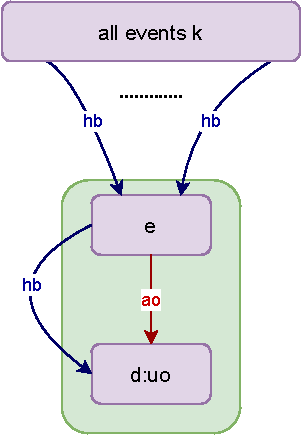
\includegraphics[scale=0.7]{InstructionReordering/Lemmas/lemma_proof1_case1.pdf}
        \caption{For the first case}
        \label{fig:my_label}
    \end{figure}
    
    In the second case,
    \[
        \et{d}{sc} \wedge d\!\in\!W
        \tag{4}
        \label{l14}
    \]
    
    Then for any event $k$
    \[
        dir(k,d) \Rightarrow cons(k,d)
        \qquad from \quad
        (\ref{l14})
        \tag{5}
        \label{l15}
    \]
    
    We once again have event $e$ satisfying the above
    \[
        k = e 
        \qquad from \quad
        (\ref{l10}, \ref{l15})
        \tag{6}
        \label{l16}
    \]
    
    Though there could be direct \textit{happens-before} relation with some event $k$ from another \textit{agent}, these are only relations satisfying $dir(d,k)$. Thus, we can once again infer that for any $k \neq e$ 
    
    \[
        \reln{k}{hb}{d} \Rightarrow \reln{k}{hb}{d}
        \qquad from \quad
        (\ref{l10}, \ref{l14}, \ref{l15}, \ref{l16})
    \]
    
    The following figure explains this intuition: 
    
    \begin{figure}[H]
        \centering
        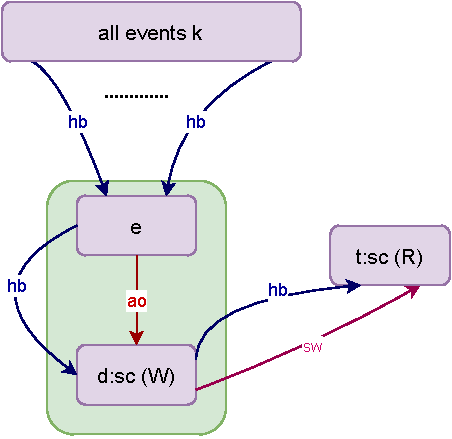
\includegraphics[scale=0.7]{InstructionReordering/Lemmas/lemma_proof1_case2.pdf}
        \caption{For the second case}
        \label{fig:my_label}
    \end{figure}
    
\end{proof}

%---------------------------------------------------------------------------------------------------------------    

%SHORTER VERSION OF PROOF WITHOUT THE ENGLISH EXPLAINATION IN THE MIDDLE. DISCUSS AND DECIDE ON WHICH FORM IS BETTER
\begin{lemma}Consider three events $e$, $d$ and $k$ \\

    If
        
        \[
            \cons{e}{d} \ \wedge \ \reln{e}{ao}{d} \ \wedge \
            (
                (\et{e}{uo}) \ \vee \
                (\et{e}{sc} \ \wedge \ \event{e}{R})
            )
        \]
        
    then,
        \[
            \reln{e}{hb}{k} \Longrightarrow \reln{d}{hb}{k}
        \]

 When we have two consecutive events \textit{e} and \textit{d} which are one after the other (i.e. $\reln{e}{ao}{d}$), we can use \textit{transitive property} of $\stck{_{hb}}$ to infer that any event \textit{k} that \textit{happens after} \textit{d}, also \textit{happens after} \textit{e}. However, is it possible to derive that the event \textit{k happens after d} using the evidence that \textit{k happens after e} ? This lemma states the condition when this is true.

\end{lemma}

%An alternative proof for this 
\begin{proof}
    
    Just like the proof for the previous lemma, we will divide the proof for this into two cases, based on what event $e$ is. Again, for both cases, we have the following to be true:
    
    \[
        cons(e,d) \ \wedge \reln{e}{ao}{d}
        \tag{0}
        \label{l20}
    \]

   In the first case,
   
   \[
        \et{e}{uo} 
        \tag{1}
        \label{l21}
   \]
   
   Then for any event k
   
   \[
        dir(e,k) \Rightarrow cons(e,k) 
        \qquad from
        \quad (\ref{l21})
        \tag{2}
        \label{l22}
   \]
   
   The event that satisfies the above with $e$ is $d$
   \[
        k = d 
        \qquad from 
        \quad (\ref{l20}, \ref{l22})
        \tag{3}
        \label{l23}
   \]
   
   Because $\stck{_{ao}}$ is a total order, $d$ would be the only such event. This would mean that for any other event $k \neq d$
   
   \[
        \reln{e}{hb}{k} \Rightarrow \reln{d}{hb}{k}
        \qquad from 
        \quad (\ref{l20}, \ref{l21}, \ref{l22}, \ref{l23})
   \]
   %Better phrase the intuition
   The following figure should explain this intuition:  
    
    \begin{figure}[H]
        \centering
        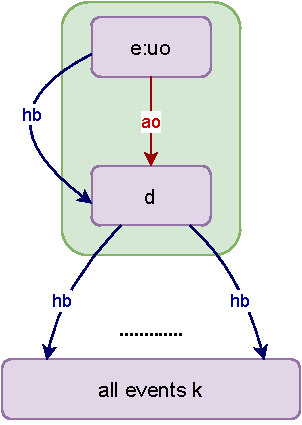
\includegraphics[scale=0.7]{InstructionReordering/Lemmas/lemma_proof2_case1.pdf}
        \caption{Caption}
        \label{fig:my_label}
    \end{figure}
    
    In the second case,
    \[
        \et{e}{sc} \wedge e\!\in\!R
        \tag{4}
        \label{l24}
    \]
    
    Then for any event $k$
    \[
        dir(e,k) \Rightarrow cons(e,k)
        \qquad from \quad
        (\ref{l24})
        \tag{5}
        \label{l25}
    \]
    
    We once again have event $d$ satisfying the above   
    \[
        k = d 
        \qquad from \quad
        (\ref{l20}, \ref{l25})
        \tag{6}
        \label{l26}
    \]
    
    Though there could be direct \textit{happens-before} relation with some event $k$ from another \textit{agent}, these are only relations satisfying $dir(k,e)$. Thus, we can once again infer that for any $k \neq d$ 
    
    \[
        \reln{e}{hb}{k} \Rightarrow \reln{d}{hb}{k}
        \qquad from \quad
        (\ref{l10}, \ref{l24},  \ref{l25}, \ref{l16})
    \]
    
    The following figure explains this intuition: 
    
    \begin{figure}[H]
        \centering
        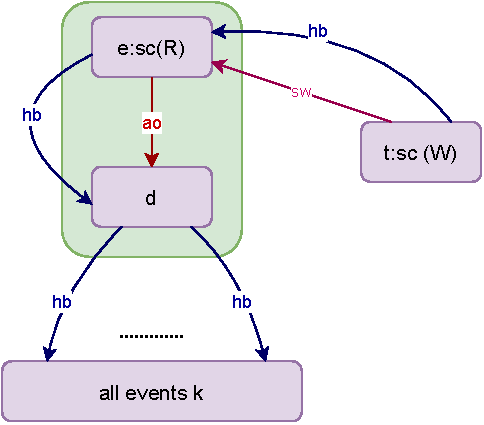
\includegraphics[scale=0.7]{InstructionReordering/Lemmas/lemma_proof2_case2.pdf}
        \caption{Caption}
        \label{fig:my_label}
    \end{figure}

\end{proof}

%------------------------------------------------------------------------------


\subsection{Valid reordering}
    We view reordering as manipulating the agent-order relation among two events. In that sense, reordering two consecutive events $e$ and $d$ such that $e \stck{_{ao}} d$ becomes:
    \[
        e \stck{_{ao}} d 
        \longmapsto
        d \stck{_{ao}} e 
    \]

    What implications this change has on the other ordering relations depends on the type of events $e$ and $d$ are and would require an analysis on each Candidate Execution. 
    The intuition is that the axioms of the memory model rely on certain ordering relations to restrict observable behaviors in a program.
    Hence, preserving these ordering relations would help us in turn not introduce new Observable Behaviors.
    In particular we note that preserving $\stck{_{hb}}$ relations (other than the one we eliminate intentionally i.e $\reln{e}{hb}{d}$) would suffice for our purpose. 
    Since $\stck{_{mo}}$ respects $\stck{_{hb}}$, we in turn even preserve the memory order which is essential.  

    In the end, we want to ensure that the set of possible observable behaviors of a program, remain unchanged after reordering. If that is not feasible, then we would want the set of observable behaviors after reordering at the very least to be a subset. This would ensure that the program does not have some new behaviours that weren't supposed to happen prior to reordering. 
    
    We begin by first defining a reorderable pair of events. We then formulate a theorem (with a proof) on the set of observable behaviors of a Candidate before and after reordering a pair of consecutive events which are reorderable. We consider reordering valid if the set of observable behaviours after reordering are a subset of the original. 

    \begin{definition}{Reorderable Pair (Reord)}
        We define a boolean function \emph{Reord} that takes two ordered pair of events $e$ and $d$ such that $\reln{e}{ao}{d}$ and gives a boolean value indicating if they are a reorderable pair. 
        
        \begin{align*}
            Reord(e,d) = \\
            (
            &((\et{e}{uo} \ \wedge \ \et{d}{uo}) \ \wedge \ 
                    (   
                        (\event{e}{R} \ \wedge \ \event{d}{R}) \ \vee \ 
                        (\Re(e) \cap_\Re \Re(d) = \phi) 
                    )
            ) \\ &\vee \\
            &((\et{e}{sc} \ \wedge \ \et{d}{uo}) \ \wedge \ 
                    (
                        (\event{e}{W} \ \wedge \ (\Re(e) \cap_\Re \Re(d) = \phi)) 
                    )
            ) \\ &\vee \\
            &((\et{e}{uo} \ \wedge \ \et{d}{sc}) \ \wedge \ 
                    (
                        (\event{d}{R} \ \wedge \ (\Re(e) \cap_\Re \Re(d) = \phi)) 
                    )
            )
            )
        \end{align*}

        \critic{purple}{Use the latter for the purpose at the end of the proof for reordering, to emphasize how we approached each case}

         
    \end{definition}

    \begin{theorem} 

    Consider a candidate $C$ of a program and its possible \textit{Candidate Executions} where $\stck{_\textit{hb}}$ is strictly partial order. Consider two events $e$ and $d$ such that $\cons{e}{d}$ is true in $C$ and  $\reln{e}{ao}{d}$. Consider another candidate $C'$ resulting after reordering $e$ and $d$. 
    Then if \emph{Reord(e,d)} is true in $C$, the set observable behaviors possible due to Candidate Executions of $C'$ is a subset of that of $C$. 
\end{theorem}


    \begin{proof}
    We look at this as an elimination of $e$ that takes place in any candidate execution of $C$. 
    We then go about answering the same four questions as we did for reordering. 
    The only major change here being that elimination implies removal $\stck{_{hb}}$ relations, in contrast to introducing new ones.
    We must check whether the removal of these relations introduce new behaviors.
    
    
\paragraph{1. Preserving \textit{happens-before} relations}
        
    If $\stck{_{hb}}$ relations among events are lost after reordering, they may introduce new observable behaviors. The relations that are subject to change can be divided into four parts using events $e$ and $d$.
    \begin{tasks}(2)
        \task $\reln{k}{hb}{e}$.
        \task $\reln{e}{hb}{k}$.
        \task $\reln{d}{hb}{k}$.
        \task $\reln{k}{hb}{d}$.
    \end{tasks}

    Firstly, note that the relations of the form $\reln{e}{hb}{k}$ come through either a $\stck{_{sw}}$ relation with $e$ or relations through event $d$, i.e. of the form $\reln{d}{hb}{k}$. 
    The ones that come due to the latter, may not be preserved after reordering. 
    Note also that, a similar argument exists for relations of the form $\reln{k}{hb}{d}$ wherein relations derived through $e$($\reln{k}{hb}{e}$) may be lost after reordering. 

    Hence, the relations that could be subject to change can be addressed by considering two disjoint sets of events in any \textit{Candidate Execution} of $C$ as below.
    \begin{align*}
       K_e = \{k \ | \ \reln{k}{hb}{e} \}. \\
       K_d = \{k \ | \ \reln{d}{hb}{k} \}. 
    \end{align*}

    Figure~\ref{reord:preserve_hb(a)} below pictorially shows this.
    \begin{figure}[H]
        \centering
        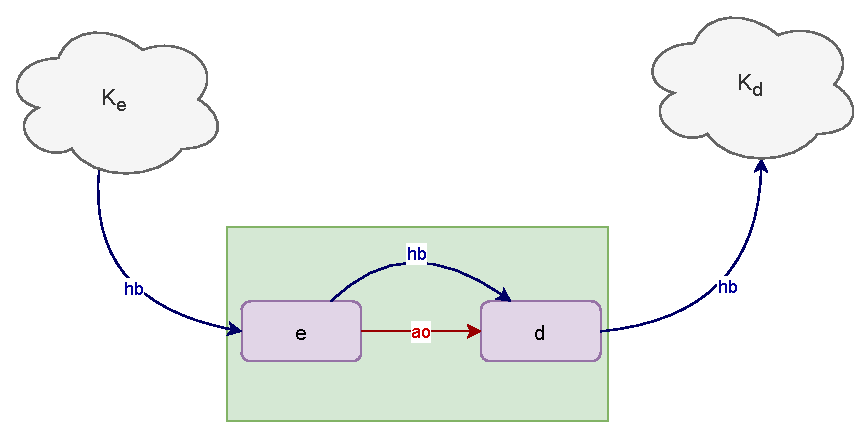
\includegraphics[scale=0.7]{4.InstructionReordering/4.ValidReorderingCandidate/ProofParts/Part1/part1(a).pdf}
        \caption{For any Candidate Execution of $C$, the set $K_e$ and $K_d$ and its relation with events $e,d$.}
        \label{reord:preserve_hb(a)}
    \end{figure}
    
    Consider two events $\event{p1}{K_e}$ and $\event{p2}{K_d}$ (When $e$ is the first event or $d$ is the last event, assume dummy events that can act as $p1$ or $p2$.) belonging to the same agent as that of $e$ and $d$ such that in $C$:
    \begin{align*}
        dir(p1,e)\ \wedge\ dir(d,p2).
    \end{align*}
    
    Note that in terms of direct happens-before relations, on reordering, any $Candidate Execution$ of $C$ will have the following changes shown in Figure~\ref{reord:preserve_hb(b)}
    \begin{figure}[H]
        \centering
        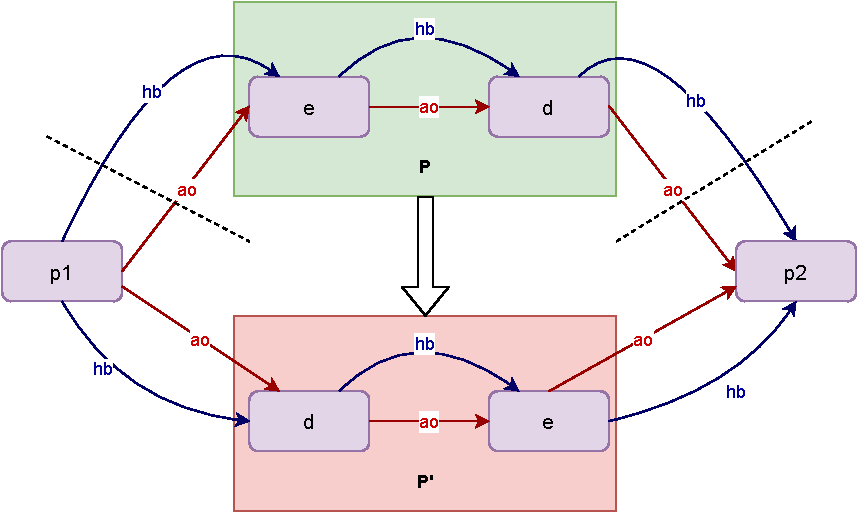
\includegraphics[scale=0.7]{4.InstructionReordering/4.ValidReorderingCandidate/ProofParts/Part1/part1(b).pdf}
        \caption{The \textit{direct happens-before} relation that change while reordering events $e$ and $d$.}
        \label{reord:preserve_hb(b)}
    \end{figure}
    
    The figure above is to show that, for any $Candidate Execution$ of $C$, the following is true
    \[
        cons(p1,e) \ \wedge dir(p1,e) \ \wedge dir(e,d) \ \wedge cons(d,p2) \ \wedge \ dir(d,p2).
    \]
    and for that of $C'$,
    \[
        cons(p1,d) \ \wedge \ dir(p1,d) \ \wedge \ dir(d,e) \ \wedge cons(e,p2) \ \wedge dir(e,p2).
    \]
    
    We need the following key relations to be preserved in Candidate executions of $C'$ 
    \begin{tasks}(2)
        \task $\reln{p1}{hb}{e}.$
        \task $\reln{e}{hb}{k}.$
        \task $\reln{d}{hb}{p2}.$
        \task $\reln{k}{hb}{d}.$ 
    \end{tasks}

    After reordering, we have (a) and (c) preserved due to transitivity  
    \begin{gather*}
        \reln{p1}{hb}{d} \ \wedge \ \reln{d}{hb}{e} \ \Rightarrow \ \reln{p1}{hb}{e}. \\
        \reln{e}{hb}{p2} \ \wedge \ \reln{d}{hb}{e} \ \Rightarrow \ \reln{d}{hb}{p2}. \\
        \reln{p1}{hb}{d} \ \wedge \ \reln{d}{hb}{e} \ \wedge \ \reln{e}{hb}{p2} \ \Rightarrow \ \reln{p1}{hb}{p2}. 
    \end{gather*}

    (b) and (d) may not be preserved due to $\reln{d}{sw}{k}$ or $\reln{k}{sw}{d}$. If we can "pivot" the  set $K_e$ to $p1$ and $K_d$ to $p2$, it would ensure that our other two intended relations also remain preserved after reordering by transitivity. To state formally, we have a valid pair of pivots $<p1,p2>$ when the following two conditions hold
    \begin{gather*}
        \forall \ k \in K_e - \{p1\}, \ \reln{k}{hb}{p1}. \\
        \forall \ k \in K_d - \{p2\}, \ \reln{p2}{hb}{k}.
    \end{gather*}
    
    By Lemma \ref{Lemma1} and \ref{Lemma2} respectively, we have for $C$, the following condition where $<p1, p2>$ is a valid pivot pair.
    \begin{gather*}
        \et{e}{uo} \vee (\et{e}{sc} \wedge \event{e}{W}). \\
        \et{d}{uo} \vee (\et{d}{sc} \wedge \event{d}{R}).
    \end{gather*}
        
    Figure~\ref{reord:preserve_hb_table} summarizes the cases where we have a valid pair of pivots\footnotemark $<p1,p2>$.
    \begin{figure}[H]
        \centering
        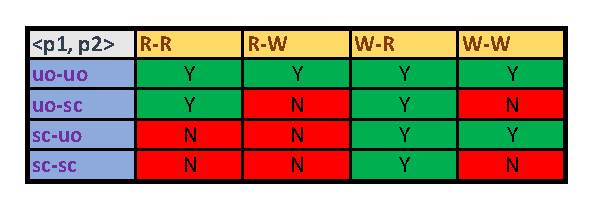
\includegraphics[scale=0.7]{4.InstructionReordering/4.ValidReorderingCandidate/ProofParts/Part1/part1_table.pdf}
        \caption{Table summarizing whether we have valid pair of pivots based on  $e$ and $d$.}
        \label{reord:preserve_hb_table}
    \end{figure}
            
    We show a simple example (Figure~\ref{reord:preserve_hb(c)} and \ref{reord:preserve_hb(d)}) where we do not have a valid pair of pivots, particularly because $p1$ is not a valid pivot. 
    Note that in this example, $K_e = K_{e1} + K_{e2} + p1 + p_x$
    \begin{figure}[H]
        \centering
        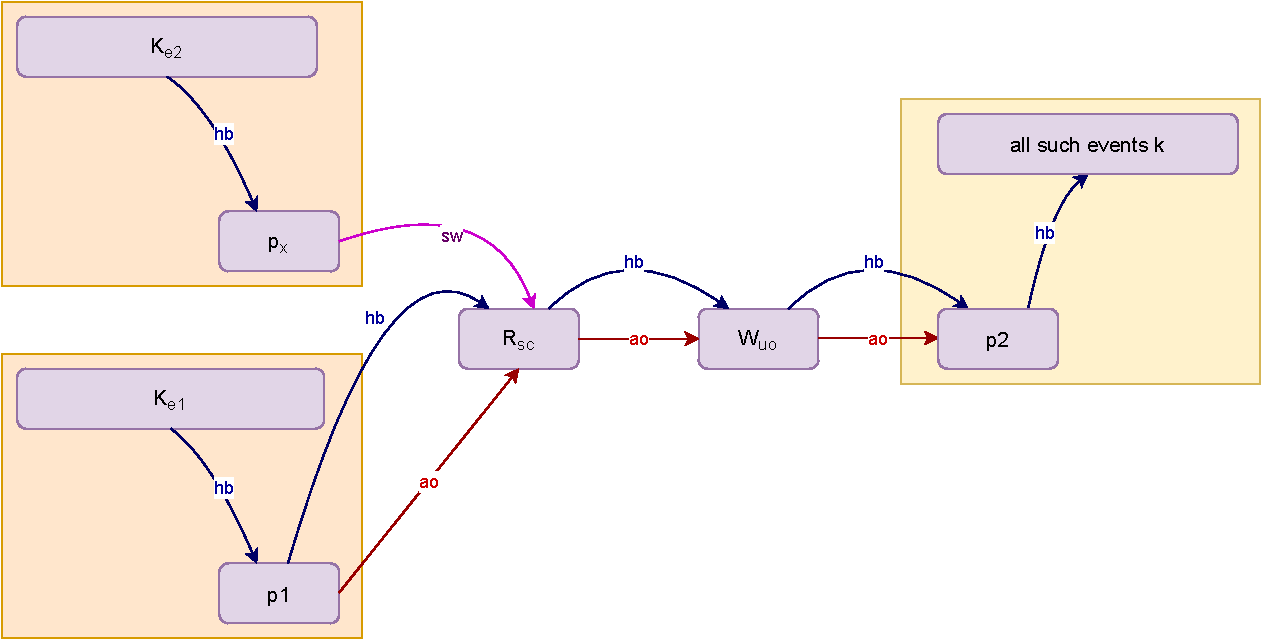
\includegraphics[scale=0.6]{4.InstructionReordering/4.ValidReorderingCandidate/ProofParts/Part1/part1(e).pdf}
        \caption{A Candidate Execution where p1 is not a valid pivot.}
        \label{reord:preserve_hb(c)}
    \end{figure}
    
    %Show figure here of program P'
    \begin{figure}[H]
        \centering
        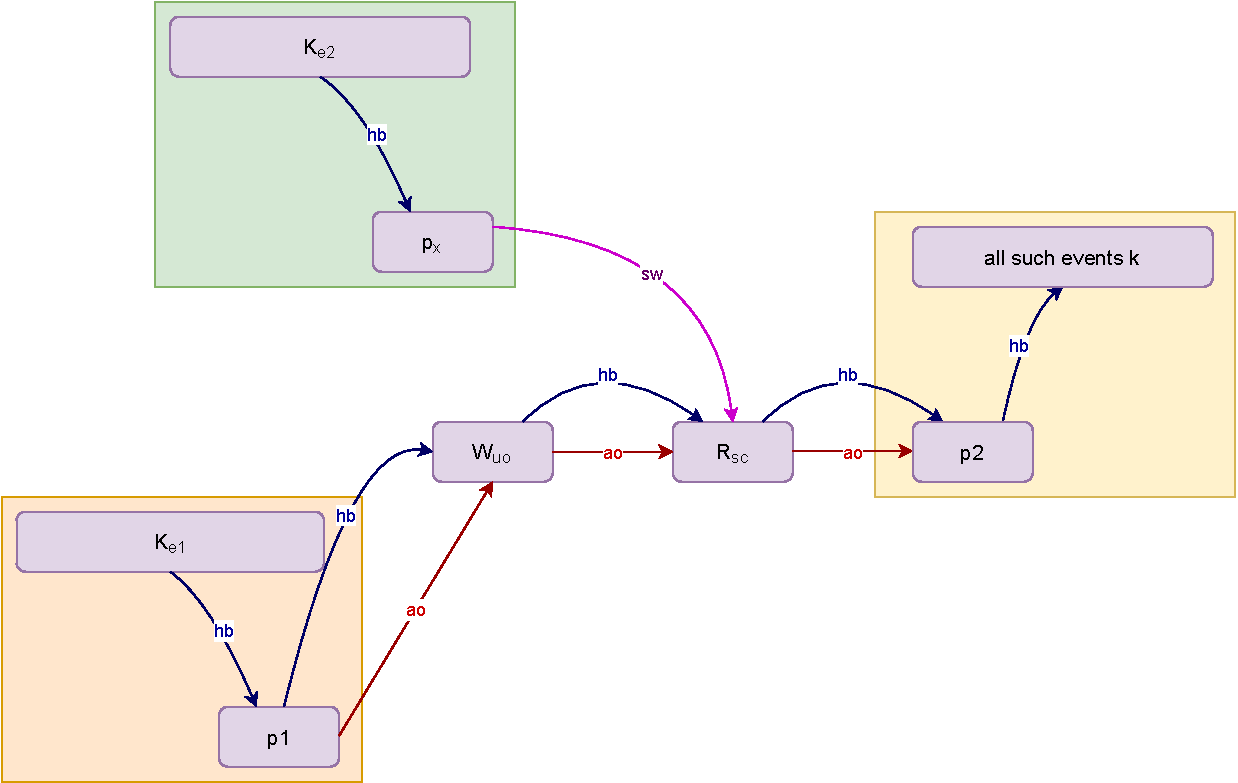
\includegraphics[scale=0.6]{4.InstructionReordering/4.ValidReorderingCandidate/ProofParts/Part1/part1(f).pdf}
        \caption{The resultant Candidate Execution after reordering, exposing the relations with $p_x$, $K_{e2}$ and $d$ that are lost}
        \label{reord:preserve_hb(d)}
    \end{figure}
        
    \footnotetext{This proof does not go about showing the exact happens-before relations that are preserved; rather it uses the properties between different happens before relations that hold, which would imply that for any possible Candidate Execution after reordering, the set of happens-before relations apart from that between $e$ and $d$ remain the same.}
    
\paragraph{2. Additional \textit{happens-before} relations}
    Although we have identified the cases when \textit{happens-before} relations are preserved, we also get some additional relations in some of them.

    %Show an example here and explain
    As an example, for the case when $d$ is a sequentially consistent read, by Lemma \ref{Lemma1}, in any execution of $C$
    \[
        \reln{k}{hb}{d} \centernot\Rightarrow \reln{k}{hb}{e}. 
    \]

    But in $Executions$ of candidate $C'$, by transitivity, we have 
    \[
        \reln{k}{hb}{d} \Rightarrow \reln{k}{hb}{e}. 
    \]

    This is because, there are \textit{happens-before} relations that come through \textit{synchronize-with} relations with $d$. 
    Thus, although we are able to preserve relations that existed in any $Candidate Execution$ of $C$, we also in the process, introduce new ones in $Candidate Executions$ of $C'$. 
    Figures~\ref{reord:add_reln(a)} and \ref{reord:add_reln(b)} shows pictorially an example of a Candidate Execution of $C$ for the case above 
    \begin{figure}[H]
        \centering
        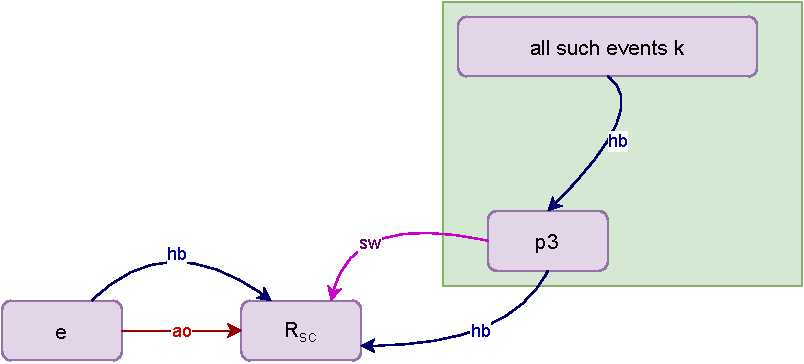
\includegraphics[scale=0.7]{5.InstructionReordering/4.ValidReorderingCandidate/ProofParts/Part2/part2(c).pdf}
        \caption{A Candidate Execution where $d$ read having access mode $sc$.}
        \label{reord:add_reln(a)}
    \end{figure}

    %Show figure here of program P'
    \begin{figure}[H]
        \centering
        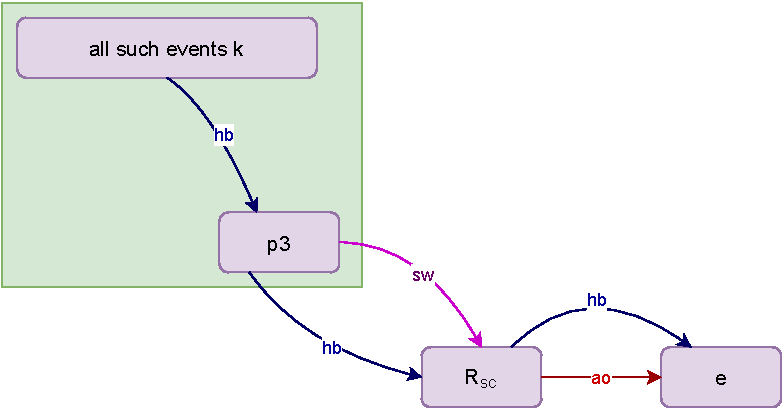
\includegraphics[scale=0.7]{5.InstructionReordering/4.ValidReorderingCandidate/ProofParts/Part2/part2(d).pdf}
        \caption{The Candidate Execution after reordering $e$ and $d$, exposing the new relations established with $e$, $p3$ and set $k$}
        \label{reord:add_reln(b)}
    \end{figure}

    Figure~\ref{reord:add_reln_table} below shows the cases where new relations could be introduced. 
    \begin{figure}[H]
        \centering
        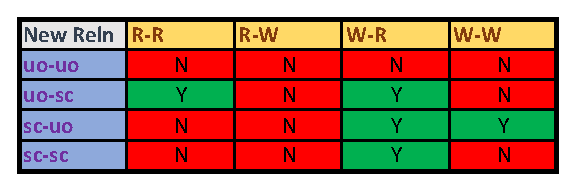
\includegraphics[scale=0.7]{5.InstructionReordering/4.ValidReorderingCandidate/ProofParts/Part2/part2_table.pdf}
        \caption{Table summarizing new \textit{happens-before} relations that could be introduced on having valid pair of pivots.}
        \label{reord:add_reln_table}
    \end{figure}

    For these cases, we investigate whether the new relations introduce new observable behaviors. 

    \paragraph{3. Presence of Cycles?}
        
Because no new $\stck{_{hb}}$ relations are introduced, and because original candidate executions have $\stck{_{hb}}$ as a strict partial order, no cycles are introduced after elimination. 


    \paragraph{4. Do the lost relations result in New Observable Behaviors?}

        To answer this, we need to see whether the relations removed had an impact on $\stck{_{rf}}$ relations other than those with $e$. To prove that it does not have any impact, we divide our argument into two parts, viz. into the two types of relations removed:

        \begin{tasks}(2)
            \task $\reln{k}{hb}{R_uo}$ 
            \task $\reln{R_uo}{hb}{k}$ 
        \end{tasks}

        In the first case, we have the following possibilities. 
        \begin{figure}[H]
            \centering
            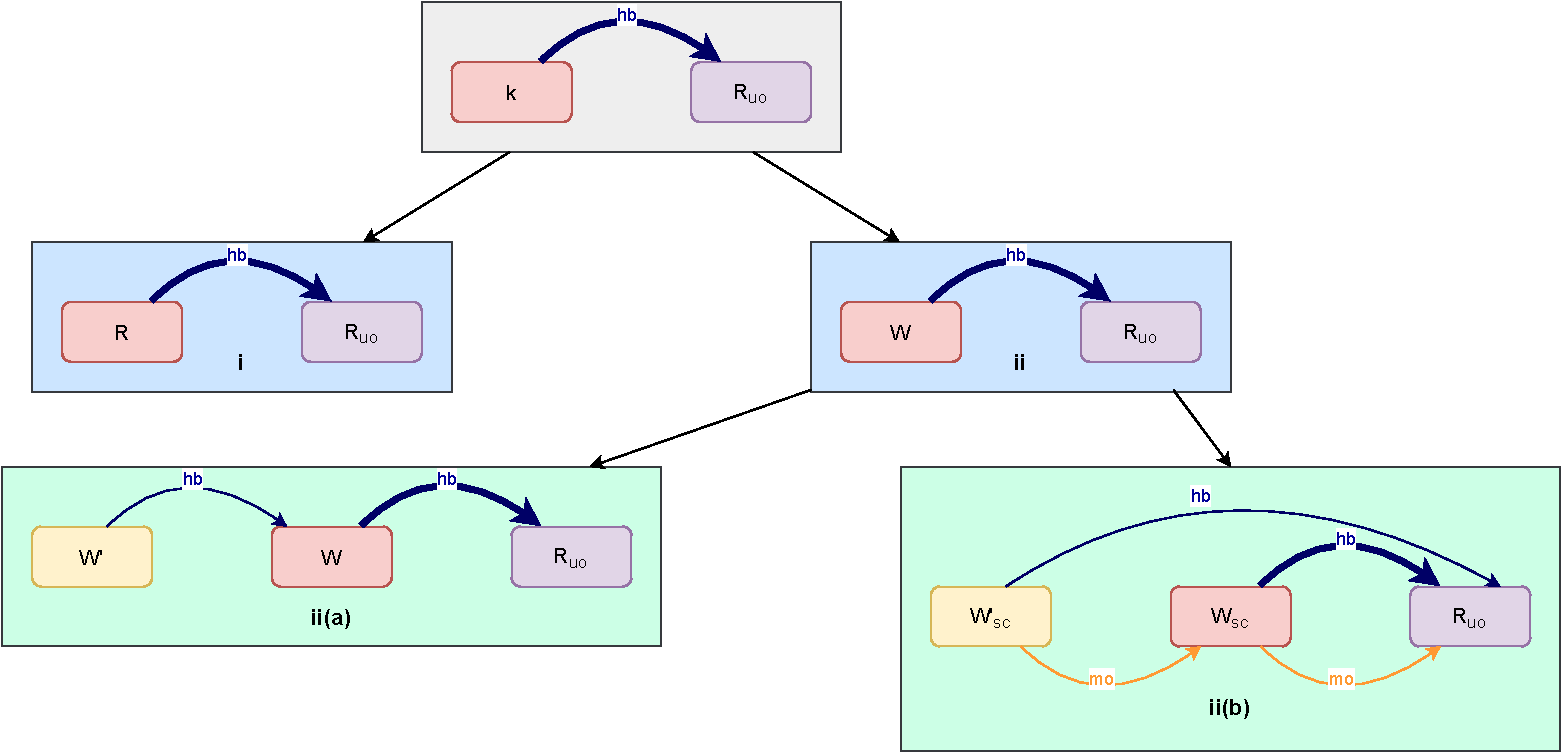
\includegraphics[scale=0.5]{6.Elimination/1.ValidEliminationCandidate/ReadElimProof/ProofParts/Part4_Case1.pdf}
            \caption{The first type of relations removed and the various patterns forbidden by them.}
        \end{figure}

        Observations:
        \begin{itemize}
            \item (i) is not a pattern forbidden by the consistency rules.
            \item (ii)(a) is a pattern of Axiom \ref{CoRe}, however, only restricting $\stck{_{rf}}$ relation with $R$ and $W'$(which here is our Unordered Read)
            \item (ii)(b) is a pattern of Axiom \ref{SeqCsAt}, however, once again, only restricting $\stck{_{rf}}$ relation with $R$ and $W'$. 
        \end{itemize}

        In the second case, we have the following possibilites.
        \begin{figure}[H]
            \centering
            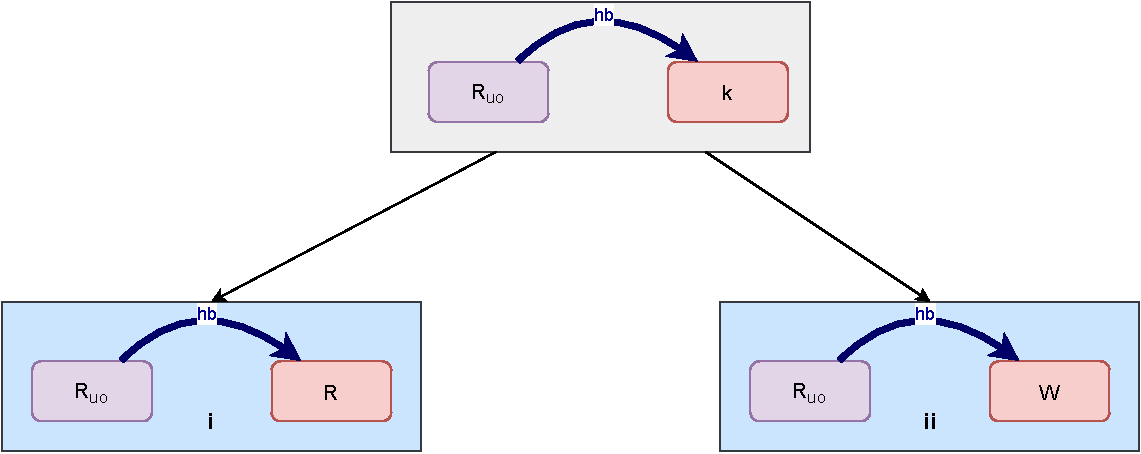
\includegraphics[scale=0.5]{6.Elimination/1.ValidEliminationCandidate/ReadElimProof/ProofParts/Part4_Case2.pdf}
            \caption{The second type of relations removed and the various patterns forbidden by them.}
        \end{figure}

        Observations:
        \begin{itemize}
            \item (i) is not a pattern in any Consistency rules
            \item (ii) is a pattern of Axiom \ref{CoRe}, however, only restricting $\stck{_{rf}}$ relation with $R$ and $W$
        \end{itemize}

        From the above observations, we can infer that the relations removed only have restriction on reads-from relations on the event $e$ we eliminate. Thus, we can conclude that no new observable behaviors are introduced due to the removed $\stck{_{hb}}$ relations. 
    
\end{proof}

    \begin{corollary}
    Consider a Candidate C of a program and its Candidate Executions which are valid. Consider two write events $e$ and $d$ both having equal ranges such that $\neg \cons{e}{d}$ is true in C, $e$ is of type unordered and $\reln{e}{ao}{d}$. 
    Consider another Candidate C' without the event $e$.  
    Then, the set of Observable behaviors possible in C' is a subset of C only if the following holds true.
    \begin{align*}
        \forall \ i \ \in \ [1,n-1] \ \textit{s.t.} \
        \reln{e}{ao}{k_1} \ \wedge \ \reln{k_n}{ao}{d} \ \wedge \ \reln{k_i}{ao}{k_{i+1}} \ \wedge \  
        \cons{e}{k_1} \ \wedge \ \cons{k_n, d} \ \wedge \ \cons{k_i, k_{i+1}}, \\
        \exists \ (n + 1) \geq j > 0 \ \textit{s.t.} \ 
        \forall l \ \in \ [1,j-1] \ . \ Reord(e, k_l) \ 
        \wedge \ 
        \forall m \ \in \ [j,n] \ . \ Reord(k_m, d) 
    \end{align*}
            
    
\end{corollary}

\begin{proof}

    We prove this using induction on the number of events $k$ between $e$ and $d$. For each case, we see whether a valid $j$ exists. 

    \paragraph{Base Case (n=1)}

        For this case, if we have $Reord(e,k1)$ then $j=2$ is a valid choice. By Theorem of reordering, we get Candidate $C''$ with $\cons(e,d)$ whose observable behaviors are a subset. By Theroem (write elim), a observable behaviors of $C'$ is a subset of that of $C''$. By transitivity property of subsets, behaviors of $C'$ is a subset of $C$. 
        
        \critic{blue}{Write above arguments properly}
    
        While if we have $Reord(k1,d)$ then $j=1$ is a valid choice. The argument is the same as above. 
        
    \paragraph{Inductive Case (n)}
        
        Suppose the corollary holds for the case $n$. Meaning, the observable behaviors of $C'$ is a subset of $C$. And suppose $j$ is alos the number as needed. 

        Then for the case where there are $n+1$ events,we have the following two cases:

        If $k_x$ is the additonal event added in between $e$ and $d$, then, if $Reord(k_x, d) \wedge x>j$, the new $j$ remains the same as the old one. Because $Reord(K_{n+1}, d)$, by theorem of reordering, the Candidate $C''$ after reordering has observable behaviors as a subset of $C$. Now after reordering, we have our inductive case assumption, hence observable behaviors of $C'$ is a subset of $C$. 
        
        On the other hand, if $Reord(e,k_x) \wedge x \leq j$, the new $j$ is plus one the old $j$. Because $Reord(e,k_1)$  by theorem of reordering $e$ and $k_1$, the Candidate $C''$ after reordering has observable behaviors as a subset of $C$. Now $j$ for $C''$ becomes $j-1$, hence we get our original inductive case assumption on $n$. By transitive property of subsets observable behaviors of $C'$ is a subset of $C$. 

        \critic{red}{Very rudimentary format of arguments, discuss with Clark and get them more formal}

    
\end{proof}

\begin{proof}
    We prove by induction on the number of events $k$ between $e$ and $d$. We verify that if a $j$ exists that is valid, the Observable behaviors of $C'$ is a subset of $C$.

    \paragraph{Base Case : n = 1}

        We have the case when:
        \begin{align*}
            \reln{e}{ao}{k_1} \ \wedge \ reln{k_1}{ao}{d}
        \end{align*}
        We can divide this into two cases one with $Reord(e, k_1)$ and one with $Reord(k_1, d)$.

        In the first case, note that $j=2$ is the valid choice. Thus, by Theorem of Reordering and Def of consecutive events and agent order, we can reorder $e$ and $k_1$, thus giving us a Candidate $C''$ with :
        \begin{align*}
            \reln{k_1}{ao}{e} \ \wedge \ \reln{e}{ao}{d}
        \end{align*}  
        whose observable behaviors are a subset of $C$

        Due to Def of Consecutive instructions and Theorem of Elmination, we can eliminate $e$, thus giving us 
        \begin{align*}
            \reln{k_1}{ao}{d}
        \end{align*} 

\end{proof}


\subsection{Counter examples for the invalid cases}

\subsection{}

    

    
    
    
    
    

%The end ? ------------------------------------------------------------------------------------------------------------------------------    
    
\end{document}
